\section{基地駐守 (base)}

\textcolor{red}{\textbf{本題有 Special Judge,會依照解的好壞程度動態給分。}}

\subsection{問題描述}

烏克麗麗王國的領土以一個無向圖 (undirected graph) 來代表,圖上的每個頂點
(vertex) 代表一個基地,而圖上的邊 (edge) 為連接基地與基地之間的道路。
領土中的基地編號為 \(1\) 到 \(n\),每一條基地間的道路距離都恰好為 \(1\)
單位,並且城巿 \(i\) 一開始有駐守 \(w_i\) 單位的守軍。
當一個城巿裡\textbf{恰好}有 \(S\)
個單位的守軍駐守時,此基地達到完美防守的狀態,能抵擋任何外來的攻擊。
由於烏克麗麗王國即將面臨外敵的侵略,在此問題中,你的目標是協助移動烏克麗麗王國各基地的守軍,讓最多個城巿達到完美防守的狀態。

由於烏克麗麗王國在歷史上長期受到外敵的威脅,他們早已未雨綢繆地在軍隊的配置上下了不少工夫。
國防大臣告訴你,在每個城巿的距離為 \(1\) 的範圍內,都至少有 \(S\)
單位的守軍。 也就是說如果將基地 \(u, v\) 的最短距離以 \(d(u, v)\)
表示的話,對任何的城巿 \(v\) 而言,以下不等式

\[\sum_{u:d(u,v) \le 1} w_u \ge S\]

\noindent 都成立。

為了避免守軍移動疲憊,烏克麗麗王國的國防大臣希望每單位守軍最長的移動距離不超過
\(X\)。 下圖為兩個 \(S = 10, X = 3\)
的例子,圖上每個圓圈代表一個基地,圓圈裡的數字代表當時基地中的守軍數量。
在圖 (a)
的例子中我們可以將右下角基地的軍隊移至上方及左下方的基地,最終結果如圖
(b) 有 \(2\) 個基地達到完美防守的狀態。 在圖 (c)
的例子中我們將左上、右下程式的軍隊分別移至其他兩個點,最終結果如圖 (d)
所示,一樣有 \(2\) 個基地為完美防守。 上面兩例子中最長的移動距離都不超過
\(3\),滿足國防大臣的希望。

\begin{minipage}{0.24\textwidth}
  \begin{figure}[H]
    \centering
    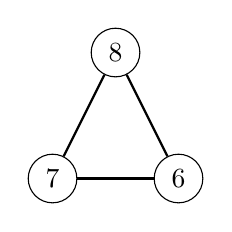
\begin{tikzpicture}[scale=0.8]
      \def \Nodes {
        1/1/2/8,
        2/0/0/7,
        3/2/0/6}
      \def \Edges {
        1/2,
        2/3,
        3/1}

      \foreach \id / \x / \y / \w in \Nodes {
        \node[draw,circle] (\id) at (\x, \y) {\w};
      }
      \foreach \x / \y / \w / \labelpos in \Edges {
        \path[draw,-,thick] (\x) -- (\y);
      }
    \end{tikzpicture}
    \caption{(a)}
  \end{figure}
\end{minipage}
\begin{minipage}{0.24\textwidth}
  \begin{figure}[H]
    \centering
    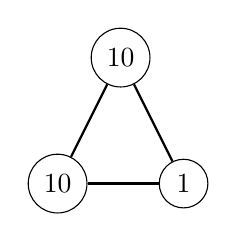
\begin{tikzpicture}[scale=0.8]
      \def \Nodes {
        1/1/2/10,
        2/0/0/10,
        3/2/0/1}
      \def \Edges {
        1/2,
        2/3,
        3/1}

      \foreach \id / \x / \y / \w in \Nodes {
        \node[draw,circle] (\id) at (\x, \y) {\w};
      }
      \foreach \x / \y / \w / \labelpos in \Edges {
        \path[draw,-,thick] (\x) -- (\y);
      }
    \end{tikzpicture}
    \caption{(b)}
  \end{figure}
\end{minipage}
\begin{minipage}{0.24\textwidth}
  \begin{figure}[H]
    \centering
    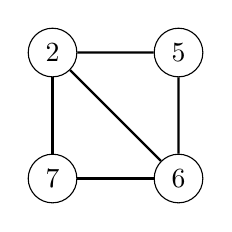
\begin{tikzpicture}[scale=0.8]
      \def \Nodes {
        1/0/0/7,
        2/2/0/6,
        3/2/2/5,
        4/0/2/2}
      \def \Edges {
        1/2,
        2/3,
        3/4,
        4/1,
        2/4}

      \foreach \id / \x / \y / \w in \Nodes {
        \node[draw,circle] (\id) at (\x, \y) {\w};
      }
      \foreach \x / \y / \w / \labelpos in \Edges {
        \path[draw,-,thick] (\x) -- (\y);
      }
    \end{tikzpicture}
    \caption{(c)}
  \end{figure}
\end{minipage}
\begin{minipage}{0.24\textwidth}
  \begin{figure}[H]
    \centering
    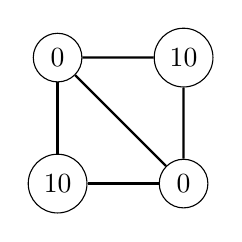
\begin{tikzpicture}[scale=0.8]
      \def \Nodes {
        1/0/0/10,
        2/2/0/0,
        3/2/2/10,
        4/0/2/0}
      \def \Edges {
        1/2,
        2/3,
        3/4,
        4/1,
        2/4}

      \foreach \id / \x / \y / \w in \Nodes {
        \node[draw,circle] (\id) at (\x, \y) {\w};
      }
      \foreach \x / \y / \w / \labelpos in \Edges {
        \path[draw,-,thick] (\x) -- (\y);
      }
    \end{tikzpicture}
    \caption{(d)}
  \end{figure}
\end{minipage}

現在你收到國防大臣的依賴,他們希望你給出一連串的軍隊移動計畫,目標是使最多數目的城巿達到完美防守並且盡可能讓軍隊最長的移動距離滿足大臣的要求。
在收到你的移動計畫後,他們會命令軍隊一起移動並在最短的時間內前往防守位置。
本題將依照輸出解滿足條件的程度動態給分,詳情請見「評分說明」一節敘述。

\subsection{輸入格式}

\begin{format}
\f{
$n$ $m$ $S$ $X$
$w_1$ $w_2$ $\cdots$ $w_n$
$u_1$ $v_1$
$u_2$ $v_2$
$\vdots$
$u_m$ $v_m$
}
\end{format}

\begin{itemize}
\tightlist
\item
  \(n\), \(m\) 分別代表王國中的基地以及道路數量。
\item
  \(S\) 代表一個基地達成完美防守恰好所需的守軍數量。
\item
  \(X\) 代表軍隊一天最長能移動的距離。
\item
  \(u_i\), \(v_i\) 為兩基地編號,代表第 \(i\) 條道路連接基地 \(u_i\) 與
  \(v_i\)。
\end{itemize}

\subsection{輸出格式}

\begin{format}
\f{
$K$ $X_a$ $O$
$a_1$ $b_1$ $c_1$
$a_2$ $b_2$ $c_2$
$\vdots$
$a_O$ $b_O$ $c_O$
}
\end{format}

\begin{itemize}
\tightlist
\item
  \(K\), \(X_a\)
  為兩整數,分別代表你輸出的移動方案中滿足完美防守的基地數以及軍隊最長移動距離。若不需要做任何移動,\(X_a\)
  請輸出 \(0\)。
\item
  \(O\) 為輸出的移動操作數量。
\item
  \(a_i\), \(b_i\), \(c_i\) 代表第 \(i\)
  個操作,會將\textbf{移動前原本在} \(a_i\) 基地的守軍 \(c_i\)
  單位移動到 \(b_i\) 基地。
\end{itemize}

\subsection{測資限制}

\begin{itemize}
\tightlist
\item
  \(1 \le n \le 500\)。
\item
  \(n-1 \le m \le \frac{n(n-1)}{2}\)。
\item
  \(1 \le S \le 500\)。
\item
  \(0 \le w_i \le 500\)。
\item
  \(5 \le X \le 500\)。
\item
  \(1 \le u_i, v_i \le n\)。
\item
  輸入的圖保證連通,沒有重邊、自環;且每個點與其相鄰點的軍隊總和
  \(\ge S\)。
\item
  以上變數皆為整數。
\end{itemize}

\subsection{評分說明}

每筆輸入檔皆有一個 \(K^{*}\)
代表所有操作中可能達到最多的完美防守基地數量。令

\begin{itemize}
\tightlist
\item
  \(K_{\Delta} = K - K^{*}\),也就是輸出的解完美防守基地數比最佳解多幾個
\item
  \(X_{\Delta} = \min\{0, X_a - X\}\),也就是輸出解的最長移動距離比大臣要求多多少
\end{itemize}

則該筆測試資料的得分為:

\[\frac{1}{1.5^{K_{\Delta}} \times 3^{X_{\Delta}}}\]

乘以該筆子任務配分,並且該子任務的得分為所有輸入檔最小的得分。請注意若有以下情況則該筆輸入以
\(0\) 分計:

\begin{itemize}
\tightlist
\item
  \(O > 500n\)
\item
  所有移動結束後,滿足完美防守的基地數量或移動最長距離不滿足輸出宣稱的
  \(K\), \(X_a\)
\item
  輸出的基地編號不存在
\item
  移動不合法,例如 \(a_i = b_i\),或者 \(c_i \le 0\)。
\item
  從基地 \(x\) 出發的的守軍單位總和比 \(w_x\) 多(沒軍隊可以移動)
\item
  不滿足輸出格式,例如有多餘非空白字元的輸出
\end{itemize}

\subsection{範例測試}

\begin{example}
\exmp{
3 3 10 5
8 7 6
1 2
2 3
3 1
}{%
2 1 2
3 1 2
3 2 3
}%
\exmp{
4 5 10 5
2 7 6 5
1 2
2 3
3 4
4 1
1 3
}{%
2 1 3
1 2 2
3 2 1
3 4 5
}%
\end{example}

\subsection{評分說明}

本題共有五組子任務,條件限制如下所示。
每一組可有一或多筆測試資料,取該組所有測試資料中最低分為該子任務得分。

\begin{longtable}[]{@{}ccl@{}}
\toprule
子任務 & 分數 & 額外輸入限制 \\
\midrule
\endhead
1 & \(4\) & 給定的圖為一條直線 \\
2 & \(20\) & 給定的圖為一棵樹 \\
3 & \(11\) & \(X \ge 20\) \\
4 & \(32\) & \(X \ge 7\) \\
5 & \(33\) & 無額外限制 \\
\bottomrule
\end{longtable}

備註:

\begin{itemize}
\tightlist
\item
  直線: 一個連通無向圖,除兩點度數為 \(1\) 以外其餘點的度數皆為 \(2\)
\item
  樹:一個連通且無環的無向圖
\end{itemize}

\section{自行車歸位 (bicycle)}

\subsection{問題描述}

在一條觀光大道上有提供免費自行車以及自行車的停車位,遊客可以隨意借用。
許多遊客在使用後並未將自行車歸位,在繁忙的一天結束後,有許多自行車散落在觀光大道的路邊,現在的任務是要將每一台自行車放置到一個停車位。

已知有 \(n\) 台自行車以及 \(m\)
個自行車的空位(\(n \le m\)),所有的自行車都是一樣的,因此任何一台自行車都可以放在任何一個空車位。
但每個自行車空位僅能停放一台自行車。
園長的困難是必須決定如何移動自行車以便最小化總移動成本,自行車與車位的位置皆以觀光大道起點的距離表示,
我們可以用一維座標來表示任何自行車以及空位的位置(以下簡稱座標)。
已知將一台自行車從座標 \(p\) 移到座標 \(q\) 的停車位所需要的成本為
\(|p – q|\)。

舉例來說,\(n = 3\) 而 \(m = 3\),自行車的座標各為
\(1, 3, 6\),而空車位的座標為 \(0, 4, 7\)。
成本最小的移動方式為:(以下用 \(x\) → \(y\) 表示將座標 \(x\)
的自行車移動到座標 \(y\) 的停車位)

\begin{itemize}
\tightlist
\item
  \(1\) → \(0\)
\item
  \(3\) → \(4\)
\item
  \(6\) → \(7\)
\end{itemize}

總成本為 \(|1 – 0| + |3 – 4| +|6 – 7| = 3\)。

\subsection{輸入格式}

\begin{format}
\f{
$n$ $m$
$a_1$ $a_2$ $\cdots$ $a_n$
$b_1$ $b_2$ $\cdots$ $b_m$
}
\end{format}

\begin{itemize}
\tightlist
\item
  \(n\), \(m\) 分別代表自行車以及停車位的數量。
\item
  \(a_i\) 為第 \(i\) 台自行車的座標。
\item
  \(b_i\) 為第 \(i\) 個停車位的座標。
\end{itemize}

\subsection{輸出格式}

\begin{format}
\f{
$D$
$c_1$ $d_1$
$c_2$ $d_2$
$\vdots$
$c_n$ $d_n$
}
\end{format}

\begin{itemize}
\tightlist
\item
  \(D\) 為最小的移動總距離
\item
  \(c_i\), \(d_i\) 代表達成最小移動總距離的方法中,要將位置在 \(c_i\)
  的自行車移動到 \(d_i\) 的停車位。
\end{itemize}

你可以輸出任何一種達成最小總距離的移動方案,但必須合法。
若有自行車重複輸出、停車位被重複使用,或者距離總和不符等情況,該筆測資以
\(0\) 分計。

\subsection{測資限制}

\begin{itemize}
\tightlist
\item
  \(1 \le n \le m \le 10^5\)。
\item
  \(0 \le a_i \le 10^9\)。
\item
  \(0 \le b_i \le 10^9\)。
\item
  所有座標皆為相異,亦即
  \(\{a_1, a_2, \cdots, a_n, b_1, b_2, \cdots, b_m\}\) 共有 \(n+m\)
  個相異整數。
\item
  以上變數皆為整數。
\end{itemize}

\subsection{範例測試}

\begin{example}
\exmp{
3 3
3 1 6
4 0 7
}{%
3
1 0
3 4
6 7
}%
\exmp{
4 4
3 4 5 6
1 2 7 8
}{%
8
3 1
4 2
5 7
6 8
}%
\end{example}

\subsection{評分說明}

本題共有四組子任務,條件限制如下所示。
每一組可有一或多筆測試資料,該組所有測試資料皆需答對才會獲得該組分數。

\begin{longtable}[]{@{}ccl@{}}
\toprule
子任務 & 分數 & 額外輸入限制 \\
\midrule
\endhead
1 & \(15\) & \(m \le 10\) \\
2 & \(16\) & \(m \le 100\) \\
3 & \(5\) & \(m \le 2000\) \\
4 & \(64\) & 無額外限制 \\
\bottomrule
\end{longtable}

\section{卡牌 (card)}

\subsection{問題描述}

A
君和他的朋友們收藏了許多桌遊卡、卡片上有許多人物如卡通人物卡、運動球員卡、明星卡等,
有些是限量發行,有些有代言人或本人親筆簽名,因此每張在遊戲中的得分也都不同。
已知每張卡片都有一個 \textbf{\(10\) 的倍數} 的得分。

今天 A 君心血來潮決定和朋友們一起玩桌遊, A
君一開始把卡牌排成一個序列,打算每一回合選一張卡片;
每一回合選出的卡片必定為未選卡牌序列的最左邊或最右邊那張。
隨著每週減少了一張卡牌,剩餘卡牌的得分就會各加上其\textbf{最初得分}的十分之一,
也就是第 \(k\) 回合結束時還未選的卡牌的得分會為最初得分的 \(1 + 0.1k\)
倍。

舉例來說,若 A 君有三張卡牌,排序後第 \(1\)、\(2\)、\(3\) 張得分分別為
\(10, 30, 20\), 若選卡順序為第 \(1\)、\(3\)、\(2\) 張,則實際得分為
\(10, 20+2, 30+3+3\) 總共為 \(68\)。 若選卡順序為第 \(3\)、\(2\)、\(1\)
張,則實際得分為 \(20, 30+3, 10+1+1\) 總共為 \(65\)。 A
君想要知道在最佳的選卡策略時,給定的卡牌序列最多可以獲得多少總得分?

\subsection{輸入格式}

\begin{format}
\f{
$n$
$S_1$ $S_2$ $\cdots$ $S_n$
}
\end{format}

\begin{itemize}
\tightlist
\item
  \(n\) 代表卡片的數量。
\item
  \(S_i\) 代表一開始 A 君預定從左到右第 \(i\) 張卡牌的得分。
\end{itemize}

\subsection{輸出格式}

\begin{format}
\f{
$S$
}
\end{format}

\begin{itemize}
\tightlist
\item
  \(S\) 為一整數,代表 A 君將卡片全選完時最多可以得到的總得分。
\end{itemize}

\subsection{測資限制}

\begin{itemize}
\tightlist
\item
  \(1 \le n \le 1000\)。
\item
  \(10 \le S_i \le 10^5\),且 \(S_i\) 必定為 \(10\) 的倍數。
\item
  以上變數皆為整數。
\end{itemize}

\subsection{範例測試}

\begin{example}
\exmp{
3
10 30 20
}{%
68
}%
\exmp{
4
20 30 50 20
}{%
143
}%
\end{example}

\subsection{評分說明}

本題共有兩組子任務,條件限制如下所示。
每一組可有一或多筆測試資料,該組所有測試資料皆需答對才會獲得該組分數。

\begin{longtable}[]{@{}ccl@{}}
\toprule
子任務 & 分數 & 額外輸入限制 \\
\midrule
\endhead
1 & \(29\) & \(n \le 20\) \\
2 & \(71\) & 無額外限制 \\
\bottomrule
\end{longtable}

\section{文字編輯器 (editor)}

\subsection{問題描述}

阿咪想要設計一款文字編輯器,能夠將特定的運算符號上色以讓使用者更容易閱讀。做為練習,阿咪先定義了合法表達式:

\begin{itemize}
\tightlist
\item
  單獨一個 \(\mathtt{x}\) 是一個合法表達式。
\item
  如果 \(e\)\hspace{0pt} 是合法表達式,則 \texttt{|}\(e\)\texttt{|}
  也是合法表達式。例如:\(\mathtt{x}\) 是合法表達式,所以
  \(\mathtt{|x|}\) 也是合法表達式。
\item
  如果 \(e\)\hspace{0pt} 是合法表達式,則 \texttt{[}\(e\)\texttt{]}
  也是合法表達式。例如:\(\mathtt{x}\) 是合法表達式,所以
  \(\mathtt{[x]}\) 也是合法表達式。
\item
  如果 \(e_1\)\hspace{0pt} 和 \(e_2\) 是合法表達式,則
  \(e_1\)\texttt{+}\(e_2\) 也是合法表達式。例如:\(\mathtt{|x|}\) 和
  \(\mathtt{[x]}\) 是合法表達式,所以 \(\mathtt{|x|+[x]}\)
  也是合法表達式。
\end{itemize}

已知:

\begin{enumerate}
\def\labelenumi{\arabic{enumi}.}
\tightlist
\item
  阿咪今天要處理的合法表達式只有 \texttt{+}, \texttt{|}, \(\mathtt{x}\)
  三種字元組成。
\item
  阿咪不小心把每條合法表達式中\textbf{恰一個} \texttt{+} 改成 \texttt{|}
  了。阿咪真是太雷了!
\item
  為了避免讓編輯器的使用者閱讀困難,阿咪決定將 \texttt{|} 全部替換成
  \texttt{[} 與 \texttt{]} 。
\end{enumerate}

但是阿咪不知道怎麼做,阿咪希望你幫她:

\begin{enumerate}
\def\labelenumi{\arabic{enumi}.}
\tightlist
\item
  把每條改壞的表達式其中一個 \texttt{|} 改成 \texttt{+}
  並且變回一個合法表達式。
\item
  將 \texttt{|} 全部替換成 \texttt{[} 與 \texttt{]}
  並且保持表達式的合法性。
\end{enumerate}

舉例來說,對於改壞的表達式
\(\mathtt{|x|||x|+|x|||}\),唯一的修復方法是將由左數來第二個 \texttt{|}
改成 \texttt{+};若以 \texttt{[} 與 \texttt{]} 取代 \texttt{|}
後,結果為 \(\mathtt{[x+[[x]+[x]]]}\)。

\subsection{輸入格式}

\begin{format}
\f{
$n$
$S_1$
$S_2$
$\vdots$
$S_n$
}
\end{format}

\begin{itemize}
\tightlist
\item
  \(n\) 代表阿咪改壞了 \(n\) 條表達式。
\item
  \(S_i\) 代表第 \(i\) 條被改壞的表達式。
\end{itemize}

\subsection{輸出格式}

\begin{format}
\f{
$O_1$
$O_2$
$\vdots$
$O_n$
}
\end{format}

\begin{itemize}
\tightlist
\item
  \(O_i\) 為一僅包含 \texttt{[]+x} \(4\) 種字元的合法表達式,將其中所有
  \texttt{[} 和 \texttt{]} 換成 \texttt{|} 後會和 \(S_i\)
  只有一個字元不同。這個不同的字元在 \(S_i\) 中是 \texttt{|};在 \(O_i\)
  中是 \texttt{+}。
\end{itemize}

若有多種可能的 \(O_i\),請輸出任何一種合乎規定的結果。

\subsection{測資限制}

\begin{itemize}
\tightlist
\item
  \(3 \le |S_i| \le 10^6\)。
\item
  \(3 \le \sum_{i=1}^n|S_i| \le 10^6\)。
\item
  \(S_i\) 只包含 \texttt{+|x} \(3\) 種字元。
\item
  對於所有 \(S_i\) ,存在一個 \texttt{|} 字元使得將其改成 \texttt{+}
  之後變成合法的表達式。
\end{itemize}

\subsection{範例測試}

\begin{example}
\exmp{
3
|x|||x|+|x|||
|x||||x|+|x||
|||||x||||x||||
}{%
[x+[[x]+[x]]]
[x]+[[x]+[x]]
[[[[[x]]+[x]]]]
}%
\end{example}

\subsection{評分說明}

本題共有四組子任務,條件限制如下所示。
每一組可有一或多筆測試資料,該組所有測試資料皆需答對才會獲得該組分數。

\begin{longtable}[]{@{}ccl@{}}
\toprule
子任務 & 分數 & 額外輸入限制 \\
\midrule
\endhead
1 & \(1\) & \(\sum_{i=1}^n|S_i| \le 20\) \\
2 & \(4\) & \(\sum_{i=1}^n|S_i| \le 300\) \\
3 & \(19\) & \(\sum_{i=1}^n|S_i| \le 2000\) \\
4 & \(76\) & 無額外限制 \\
\bottomrule
\end{longtable}

\section{齒輪組 (gears)}

\subsection{問題描述}

J老師開了一門和機器人相關的熱門選修課。
其中一個作業,是要設計一個齒輪組,用一連串的齒輪互相連接。
第一個齒輪以馬達驅動並以特定轉速轉動,目標是使最後一個齒輪輸出的轉速在一個合理範圍內,而且旋轉方向正確,這樣機器人就能以適當的速度和正確的方向移動。
任兩個相鄰的齒輪有兩種連接方式:

\begin{enumerate}
\def\labelenumi{\arabic{enumi}.}
\tightlist
\item
  接合:兩個齒輪齒對齒接在一起。前一個齒輪每轉一齒,會使下一個齒輪往相反的方向轉一齒。
\item
  帶動:兩個齒輪共用一個軸。前一個齒輪每轉一圈,會使下一個齒輪往相同的方向轉一圈。
\end{enumerate}

教室中有不同齒數的齒輪,其齒數剛巧為 \(2\) 的冪次 (如
\(8\),\(16\),\(32\) 等) 和 \(3\) 的冪次 (如 \(9\),\(27\),\(81\)
等)。
由於有不同的選擇所以每位學生做出的齒輪組長得不盡相同。請幫忙這位老師快速判斷一個齒輪組最後輸出的轉速與轉動方向,好讓他進行評分。
舉例來說,現在有一個齒輪組,包含四個齒輪,齒數依序是
\(9\)、\(8\)、\(32\)、\(16\),
且齒輪之間的連接方式依序是接合、帶動、接合。
教室的第一個齒輪固定以馬達驅動,每分鐘順時針轉 \(1\)
圈。第一個齒輪和第二個齒輪接合在一起,
因此第一個齒輪每順時針轉一圈,第二個齒輪會逆時針轉 \(1.125\) 圈。
第二個齒輪帶動第三個齒輪,因此第三個齒輪也是每分鐘逆時針轉 \(1.125\)
圈。
第三個齒輪和第四個齒輪接合在一起,因此第三個齒輪每逆時針轉一圈,第四個齒輪會順時針轉
\(2\) 圈,也就是每分鐘順時針轉 \(2.25\) 圈。
最後輸出的轉速是每分鐘順時針轉 \(2.25\) 圈。

\subsection{輸入格式}

\begin{format}
\f{
$n$
$b_1$ $e_1$ $b_2$ $e_2$ $\cdots$ $b_n$ $e_n$
$c_1$ $c_2$ $\cdots$ $c_{n-1}$
}
\end{format}

\begin{itemize}
\tightlist
\item
  第 \(i\) 個齒輪齒數為 \(b_i\) 的 \(e_i\) 次方
\item
  \(c_i = 1\) 代表第 \(i\) 和第 \(i+1\) 個齒輪為接合,若 \(c_i = 2\)
  代表為帶動。
\end{itemize}

\subsection{輸出格式}

\begin{format}
\f{
$f$ $g$ $h$
}
\end{format}

\begin{itemize}
\tightlist
\item
  \(f\) 為整數,若 \(f=1\) 代表最後一個齒輪順時針轉動,若 \(f=-1\)
  代表最後一個齒輪逆時針轉動。
\item
  \(g\),\(h\) 為兩整數,代表最後一個齒輪每一分鐘轉 \(2^g3^h\) 圈。
\end{itemize}

\subsection{測資限制}

\begin{itemize}
\tightlist
\item
  \(2 \le n \le 20\)
\item
  \(2 \le b_i \le 3\)
\item
  \(2 \le e_i \le 100\)
\item
  \(1 \le c_i \le 2\)
\item
  對 \(i \in \{1, 2, \cdots, n-2\}\),\(c_i \neq 2\) 或
  \(c_{i+1} \neq 2\) (一個軸上不會出現三個齒輪)
\item
  以上變數皆為整數。
\end{itemize}

\subsection{範例測試}

\begin{example}
\exmp{
4
3 2 2 3 2 5 2 4
1 2 1
}{%
1 -2 2
}%
\exmp{
3
2 5 2 5 2 5
1 2
}{%
-1 0 0
}%
\end{example}

\subsection{評分說明}

本題共有兩組子任務,條件限制如下所示。
每一組可有一或多筆測試資料,該組所有測試資料皆需答對才會獲得該組分數。

\begin{longtable}[]{@{}ccl@{}}
\toprule
子任務 & 分數 & 額外輸入限制 \\
\midrule
\endhead
1 & \(20\) & \(n = 2\) \\
2 & \(80\) & 無額外限制 \\
\bottomrule
\end{longtable}

\section{百萬刮刮樂 (scratchcard)}

\subsection{問題描述}

明強經營的彩券公司,近期推出百萬刮刮樂的項目。每一期百萬刮刮樂由 \(n\)
張塗有銀漆的卡片組成,分別編號 \(1, 2, 3, \cdots, n\) ,每張卡片 \(i\)
上面,由上至下依序有四筆數字 \(W_i\)、\(A_i\)、\(B_i\)、\(C_i\),其中
\(W_i\) 只有 \(3\) 種可能:\(10^6\)、\(2\times 10^6\) 或
\(3\times 10^6\)。

百萬刮刮樂的玩法如下,抽出兩張\textbf{相異}卡片 \(x\) 和
\(y\),如果這兩張卡片上面的數字同時滿足以下三個條件,那麼中獎金額就是
\(W_x + W_y\),否則就沒有中獎。

\begin{itemize}
\tightlist
\item
  條件一:\(W_x + W_y \le A_x + A_y\)
\item
  條件二:\(W_x + W_y \le B_x + B_y\)
\item
  條件三:\(W_x + W_y \le C_x + C_y\)
\end{itemize}

明強在塗銀漆之前,想查核獎項是否與廣告吻合。亦即從這群卡片中抽任 \(2\)
張相異卡片,要找出所有可能的中獎金額是多少。

\subsection{輸入格式}

\begin{format}
\f{
$n$
$W_1$ $A_1$ $B_1$ $C_1$
$W_2$ $A_2$ $B_2$ $C_2$
$W_3$ $A_3$ $B_3$ $C_3$
$\vdots$
$W_n$ $A_n$ $B_n$ $C_n$
}
\end{format}

\begin{itemize}
\tightlist
\item
  \(n\) 代表刮刮樂的數量。
\item
  \(W_i\)、\(A_i\)、\(B_i\)、\(C_i\) 代表第 \(i\) 張刮刮樂上的四個號碼。
\end{itemize}

\subsection{輸出格式}

\begin{format}
\f{
$m$
$S_1$
$S_2$
$\vdots$
$S_m$
}
\end{format}

\begin{itemize}
\tightlist
\item
  \(m\) 為一整數,代表存在幾種不同的中獎金額。
\item
  \(S_i\) 為一整數,代表第 \(i\) 小的可能的中獎金額。
\end{itemize}

\subsection{測資限制}

\begin{itemize}
\tightlist
\item
  \(1 \le n \le 2\times 10^5\)。
\item
  \(W_i \in \{10^6, 2\times 10^6, 3\times 10^6\}\)。
\item
  \(0\le A_i \le 6\times 10^6\)。
\item
  \(0\le B_i \le 6\times 10^6\)。
\item
  \(0\le C_i \le 6\times 10^6\)。
\item
  以上變數皆為整數。
\end{itemize}

\subsection{範例測試}

\begin{example}
\exmp{
3
1000000 1000001 1000001 1000002
2000000 1999999 2000002 1999998
3000000 3000001 2999998 3000001
}{%
1
3000000
}%
\exmp{
1
3000000 3000001 3000002 3000001
}{%
0
}%
\exmp{
3
2000000 0 0 0
2000000 5000000 5000000 5000000
3000000 0 0 0
}{%
2
4000000
5000000
}%
\end{example}

\subsection{評分說明}

本題共有三組子任務,條件限制如下所示。
每一組可有一或多筆測試資料,該組所有測試資料皆需答對才會獲得該組分數。

\begin{longtable}[]{@{}ccl@{}}
\toprule
子任務 & 分數 & 額外輸入限制 \\
\midrule
\endhead
1 & \(6\) & \(B_i = C_i = 3\times 10^6\) \\
2 & \(31\) & \(C_i = 3\times 10^6\) \\
3 & \(63\) & 無額外限制 \\
\bottomrule
\end{longtable}

\section{算樹 (tree)}

\subsection{問題描述}

設 \(T\) 為一棵有 \(n\) 個節點的樹,節點編號 \(1, 2, \ldots, n\),其中
\(n \ge 3\)。 \(T\) 的 Prüfer 序列可由執行以下步驟 \(n-2\) 次得到:

\begin{enumerate}
\def\labelenumi{\arabic{enumi}.}
\tightlist
\item
  找出編號最小的葉節點(即相鄰的邊數為 \(1\) 的點)\(u\),並設 \(u\) 與
  \(v\) 相鄰。
\item
  記下 \(v\) 並從 \(T\) 裡去掉 \(u\) 及邊 \(uv\)。
\end{enumerate}

\noindent 過程中依序記下的 \(n-2\) 個節點就是 \(T\) 的 Prüfer 序列。

考慮以下的樹:

\begin{figure}[h]
   \centering
   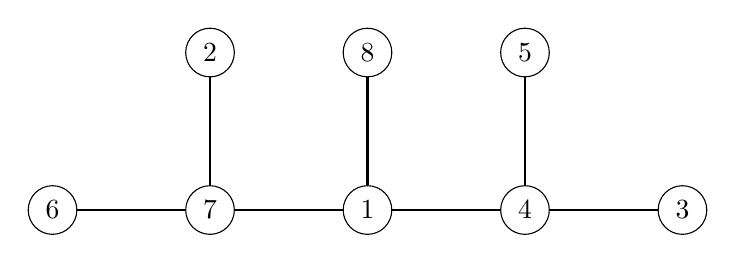
\begin{tikzpicture}
      \def \Vertices {
         1/0/0,
         2/-2/2,
         3/4/0,
         4/2/0,
         5/2/2,
         6/-4/0,
         7/-2/0,
         8/0/2}
      \def \Edges {
         1/4,
         1/7,
         1/8,
         2/7,
         3/4,
         4/5,
         6/7}
      \foreach \u / \x / \y in \Vertices {
         \node[draw, circle] (\u) at (\x, \y) {\u};
      }
      \foreach \u / \v in \Edges {
         \path[draw, thick] (\u) -- (\v);
      }
   \end{tikzpicture}
\end{figure}

\noindent 根據生成 Prüfer 序列的步驟,先將編號最小的葉節點 \(2\) 及邊
\(27\) 去掉,並記下與之相鄰的點 \(7\) 得到

\begin{figure}[h]
   \centering
   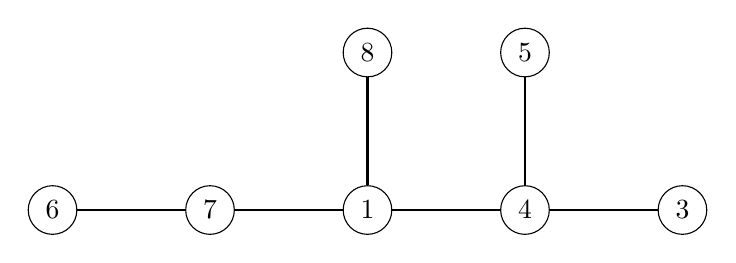
\begin{tikzpicture}
      \def \Vertices {
         1/0/0,
         3/4/0,
         4/2/0,
         5/2/2,
         6/-4/0,
         7/-2/0,
         8/0/2}
      \def \Edges {
         1/4,
         1/7,
         1/8,
         3/4,
         4/5,
         6/7}
      \foreach \u / \x / \y in \Vertices {
         \node[draw, circle] (\u) at (\x, \y) {\u};
      }
      \foreach \u / \v in \Edges {
         \path[draw, thick] (\u) -- (\v);
      }
   \end{tikzpicture}
\end{figure}

\noindent 接著再將上圖編號最小的葉節點 \(3\) 及邊 \(34\)
去掉,並記下與之相鄰的點 \(4\)。 如此重複直到最後剩下兩個點 \(1\) 與
\(8\),過程中依序記下的 \(7, 4, 4, 1, 7, 1\),即為這棵樹的 Prüfer 序列。

\begin{figure}[h]
   \centering
   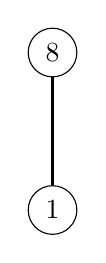
\begin{tikzpicture}
      \def \Vertices {
         1/0/0,
         8/0/2}
      \def \Edges {
         1/8}
      \foreach \u / \x / \y in \Vertices {
         \node[draw, circle] (\u) at (\x, \y) {\u};
      }
      \foreach \u / \v in \Edges {
         \path[draw, thick] (\u) -- (\v);
      }
   \end{tikzpicture}
\end{figure}

已知 \(T\) 每個節點的度數 (degree) 為 \(d_1, d_2, \ldots, d_n\),其中
\(d_i\) 為點 \(i\) 的度數,請求出 \(T\) 所有可能的 Prüfer
序列中,字典序第 \(k\) 小的。 如果 \(k\) 大於 \(T\) 可能的 Prüfer
序列數,請輸出 \(-1\)。

\subsection{輸入格式}

\begin{format}
\f{
$n$ $k$
$d_1$ $d_2$ $\ldots$ $d_n$
}
\end{format}

\begin{itemize}
\tightlist
\item
  \(n\) 代表 \(T\) 的節點數。
\item
  \(k\) 代表找出的 Prüfer 序列,字典序由小到大的排行。
\item
  \(d_i\) 代表節點 \(i\) 的度數。
\end{itemize}

\subsection{輸出格式}

如果符合條件的 Prüfer 序列有 \(k\) 個以上,請輸出

\begin{format}
\f{
$p_1$
$p_2$
$\vdots$
$p_{n-2}$
}
\end{format}

其中 \(p_1, p_2, \ldots, p_{n-2}\) 皆為整數,代表字典序第 \(k\) 小的
Prüfer 序列。否則,請輸出

\begin{format}
\f{
$-1$
}
\end{format}

\subsection{測資限制}

\begin{itemize}
\tightlist
\item
  \(3 \le n \le 10^3\)。
\item
  \(1 \le k \le 10^9\)。
\item
  \(1 \le d_i \le n-1\)。
\item
  \(d_1 + d_2 + \ldots + d_n = 2n-2\)。
\item
  以上變數皆為整數。
\end{itemize}

\subsection{範例測試}

\begin{example}
\exmp{
5 3
3 2 1 1 1
}{%
2
1
1
}%
\exmp{
4 3
1 1 2 2
}{%
-1
}%
\end{example}

\subsection{評分說明}

本題共有三組子任務,條件限制如下所示。
每一組可有一或多筆測試資料,該組所有測試資料皆需答對才會獲得該組分數。

\begin{longtable}[]{@{}ccl@{}}
\toprule
子任務 & 分數 & 額外輸入限制 \\
\midrule
\endhead
1 & \(24\) & \(n \le 8\) \\
2 & \(27\) & \(d_1 = d_2 = 1, d_3 = d_4 = \ldots = d_n = 2\) \\
3 & \(49\) & 無額外限制 \\
\bottomrule
\end{longtable}

\section{城市規劃 (ussr)}

\subsection{問題描述}

公平國最近西征得到了一塊新土地,國王打算在這塊土地上建立一座名為平等市的新城市。
為了確保所有人在公共建設議題上有平等的話語權,國王公布了平等市的城市規劃標準並開始徵稿。
身為一位城市規劃師的你,自然也想投稿看看。

平等市所在地是一片可視為二維平面的廣袤草原,上面任一點都能用 \((x, y)\)
座標表示。
國王要求城市規劃師規劃一些交通樞紐,並修築一些道路,滿足以下條件:

\begin{enumerate}
\def\labelenumi{\arabic{enumi}.}
\tightlist
\item
  交通樞紐的 \(x\) 座標與 \(y\) 座標必須是 \(0\) 到 \(10^9\)
  之間的整數,且不會有兩個交通樞紐同座標。
\item
  兩相異交通樞紐間可修築\textbf{至多一條}道路,但為了方便車輛高速行駛,修築出的道路只能是連接兩樞紐間的\textbf{最短直線線段}。
\item
  為了避免車禍,每條道路除兩端點外\textbf{不得通過其他樞紐},且任兩條道路\textbf{不得在樞紐以外之處相交}。
\item
  為了平等,每個交通樞紐都必須\textbf{恰有 \(k\) 條道路}連接。
\item
  為了住民的基礎生活品質,市內任兩個交通樞紐皆能透過道路互相抵達。
\end{enumerate}

國王要求最終規劃出來的新城市要恰有 \(n\)
個交通樞紐,請你給出一個滿足國王要求的城市規劃。
如果不存在這樣的規劃,請輸出 \(-1\)。

\subsection{輸入格式}

\begin{format}
\f{
$n$ $k$
}
\end{format}

\begin{itemize}
\tightlist
\item
  \(n\) 代表交通樞紐數。
\item
  \(k\) 代表每個交通樞紐的道路連接數。
\end{itemize}

\subsection{輸出格式}

如果存在滿足國王要求的城市規劃,請輸出

\begin{format}
\f{
$x_1$ $y_1$
$x_2$ $y_2$
\vdots
$x_n$ $y_n$
$v_{1, 1}$ $v_{1, 2}$ $\ldots$ $v_{1, k}$
$v_{2, 1}$ $v_{2, 2}$ $\ldots$ $v_{2, k}$
\vdots
$v_{n, 1}$ $v_{n, 2}$ $\ldots$ $v_{n, k}$
}
\end{format}

其中 \((x_i, y_i)\) 為交通樞紐 \(i\) 的位置,且交通樞紐 \(i\) 將會修築往
\(k\) 個相異交通樞紐 \(v_{i, 1}, v_{i, 2}, \ldots, v_{i, k}\) 的道路。
注意 \(x_i\) 與 \(y_i\) 必須是 \(10^9\) 以內的非負整數,而
\(v_{i, 1}, v_{i, 2}, \ldots, v_{i, k}\) 必須是 \(k\) 個 \(n\)
以內的相異正整數。 如果不存在這樣的城市規劃,請輸出

\begin{format}
\f{
$-1$
}
\end{format}

\subsection{測資限制}

\begin{itemize}
\tightlist
\item
  \(1 \le n \le 100\)。
\item
  \(1 \le k \le 8\)。
\item
  以上變數皆為整數。
\end{itemize}

\subsection{範例測試}

\begin{example}
\exmp{
2 1
}{%
0 0
0 1
2
1
}%
\exmp{
3 2
}{%
0 0
0 1
1 0
2 3
1 3
1 2
}%
\exmp{
4 3
}{%
0 0
1 1
1 2
2 0
2 3 4
3 4 1
4 1 2
1 2 3
}%
\exmp{
5 4
}{%
-1
}%
\exmp{
12 5
}{%
0 0
2 2
3 1
3 2
3 3
4 1
4 2
4 3
4 4
4 5
5 1
6 0
2 3 6 10 12
1 3 4 5 10
1 2 4 6 7
2 3 5 7 8
2 4 8 9 10
1 3 7 11 12
3 4 6 8 11
4 5 7 9 11
5 8 10 11 12
1 2 5 9 12
6 7 8 9 12
1 6 9 10 11
}%
\end{example}

\subsection{評分說明}

本題共有四組子任務,條件限制如下所示。
每一組可有一或多筆測試資料,該組所有測試資料皆需答對才會獲得該組分數。

\begin{longtable}[]{@{}ccl@{}}
\toprule
子任務 & 分數 & 額外輸入限制 \\
\midrule
\endhead
1 & \(4\) & \(k \le 2\) \\
2 & \(31\) & \(k \le 3\) \\
3 & \(38\) & \(k \le 4\) \\
4 & \(27\) & 無額外限制 \\
\bottomrule
\end{longtable}

\section{聖誕燈飾 (xmas)}

\subsection{問題描述}

小千買了一組 \(n\) 顆 \(m\) 色燈泡的燈飾,打算迎接即將到來的聖誕節。
這些燈泡排成一列,由左至右編號為 \(1, 2, \ldots, n\)。
燈泡的顏色是可變的,為方便起見編號為 \(1, 2, \ldots, m\)。
若一顆燈泡的顏色為 \(i\),其中 \(i \ne m\),則改變顏色會變為 \(i+1\);
若一顆燈泡的顏色為 \(m\),則改變顏色會變回 \(1\)。

每顆燈泡下皆有一個按鈕可以改變燈飾整體的顏色, 按下燈泡 \(k\)
的按鈕,會一齊改變燈泡 \(k, 2k, 3k, \ldots\) 的顏色。 例如按下燈泡 \(1\)
的按鈕,整個燈泡組的顏色都會一齊改變; 而按下燈泡 \(2\)
的按鈕,只能使編號為偶數的燈泡變色。

已知初始 \(n\) 顆燈泡的顏色分別為 \(a_1, a_2, \ldots, a_n\),
小千打算按下 \(\zeta_i\) 次燈泡 \(i\) 的按鈕,使得最後的顏色變成
\(b_1, b_2, \ldots, b_n\), 請幫她找出滿足條件的
\(\zeta_1, \zeta_2, \ldots, \zeta_n\)。 若有多組滿足條件的
\(\zeta_1, \zeta_2, \ldots, \zeta_n\),請找出字典序最小的那組;
若不存在這樣的方案,請輸出 \(-1\)。

\subsection{輸入格式}

\begin{format}
\f{
$n$ $m$
$a_1$ $a_2$ $\ldots$ $a_n$
$b_1$ $b_2$ $\ldots$ $b_n$
}
\end{format}

\begin{itemize}
\tightlist
\item
  \(n\) 代表燈泡的數量。
\item
  \(m\) 代表顏色的數量。
\item
  \(a_i\) 代表燈泡 \(i\) 的初始顏色。
\item
  \(b_i\) 代表燈泡 \(i\) 的目標顏色。
\end{itemize}

\subsection{輸出格式}

若存在滿足條件的方案,請輸出

\begin{format}
\f{
$\zeta_1$
$\zeta_2$
$\vdots$
$\zeta_n$
}
\end{format}

其中 \(\zeta_k\) 為一非負整數,代表小千應該按下燈泡 \(k\)
的按鈕次數,且字典序最小。否則,請輸出

\begin{format}
\f{
$-1$
}
\end{format}

\subsection{測資限制}

\begin{itemize}
\tightlist
\item
  \(1 \le n \le 10^6\)。
\item
  \(1 \le m \le 10^9\)。
\item
  \(1 \le a_i \le m\)。
\item
  \(1 \le b_i \le m\)。
\item
  以上變數皆為整數。
\end{itemize}

\subsection{範例測試}

\begin{example}
\exmp{
2 5
1 4
2 4
}{%
1
4
}%
\exmp{
6 10
1 1 4 5 1 4
1 2 3 4 5 6
}{%
0
1
9
8
4
2
}%
\end{example}

\subsection{評分說明}

本題共有三組子任務,條件限制如下所示。
每一組可有一或多筆測試資料,該組所有測試資料皆需答對才會獲得該組分數。

\begin{longtable}[]{@{}ccl@{}}
\toprule
子任務 & 分數 & 額外輸入限制 \\
\midrule
\endhead
1 & \(5\) & \(n \le 10, m \le 5\) \\
2 & \(27\) & \(n \le 100\) \\
3 & \(68\) & 無額外限制 \\
\bottomrule
\end{longtable}
